\begin{figure}[htbp]
\centering
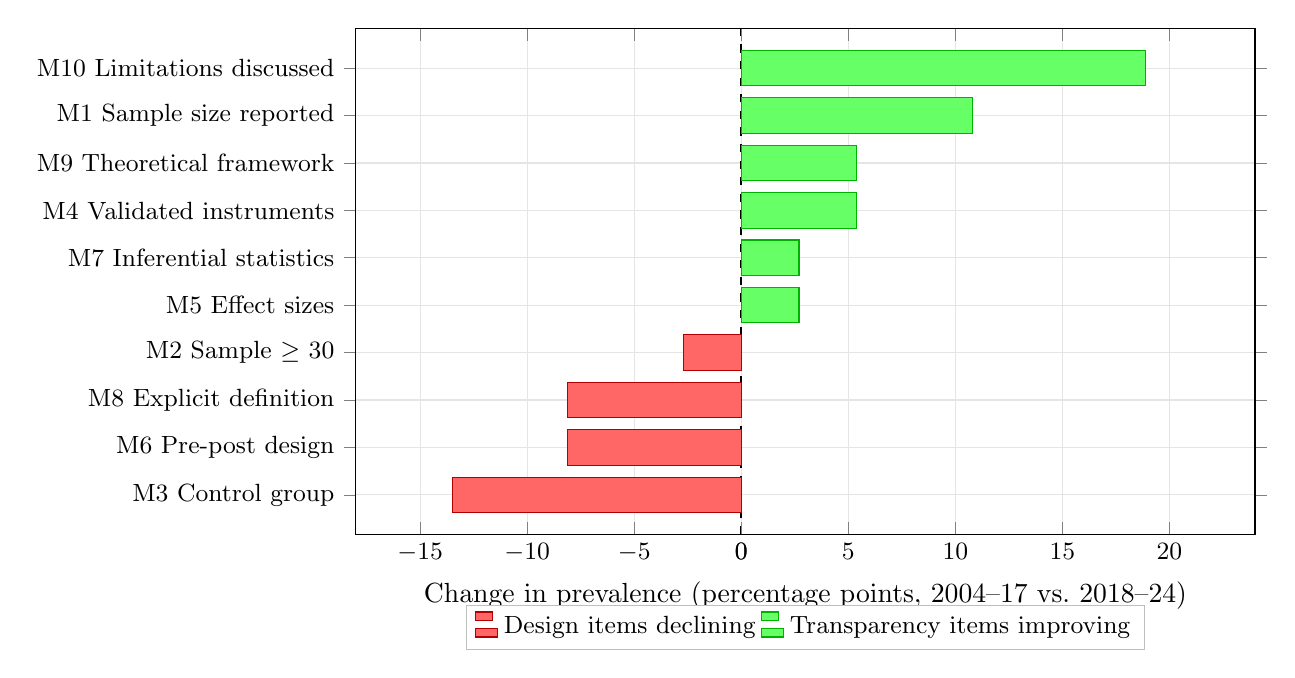
\begin{tikzpicture}
\begin{axis}[
    xbar,
    width=13cm,
    height=8cm,
    xlabel={Change in prevalence (percentage points, 2004--17 vs.\ 2018--24)},
    xmin=-18, xmax=24,
    ytick={0,1,2,3,4,5,6,7,8,9},
    yticklabels={
        {M3 Control group},
        {M6 Pre-post design},
        {M8 Explicit definition},
        {M2 Sample $\geq$ 30},
        {M5 Effect sizes},
        {M7 Inferential statistics},
        {M4 Validated instruments},
        {M9 Theoretical framework},
        {M1 Sample size reported},
        {M10 Limitations discussed}
    },
    yticklabel style={font=\small},
    xticklabel style={font=\small},
    grid=major,
    grid style={gray!20},
    bar width=0.45cm,
    extra x ticks={0},
    extra x tick style={grid=major, grid style={black, thick, dashed}},
    enlarge y limits={abs=0.5cm},
    clip=false,
    legend style={at={(0.5,-0.14)}, anchor=north, legend columns=2,
        font=\small, draw=gray!50},
]
% Negative (declining) bars — red; bar shift=0pt prevents grouping offset
\addplot[xbar, fill=red!60, draw=red!70!black, bar shift=0pt] coordinates {
    (-13.5, 0)
    (-8.1, 1)
    (-8.1, 2)
    (-2.7, 3)
};
% Positive (improving) bars — green
\addplot[xbar, fill=green!60, draw=green!70!black, bar shift=0pt] coordinates {
    (2.7, 4)
    (2.7, 5)
    (5.4, 6)
    (5.4, 7)
    (10.8, 8)
    (18.9, 9)
};
\legend{Design items declining, Transparency items improving}
\end{axis}
\end{tikzpicture}
\caption{Temporal divergence in MRQS item prevalence (2004--2017 vs.\ 2018--2024). Reporting transparency items (right, green) improved while empirical design items (left, red) declined, revealing a paradox: the field became more transparent about weaker designs.}
\label{fig:temporal-divergence}
\end{figure}
